\chapter{THỰC NGHIỆM, ĐÁNH GIÁ VÀ THẢO LUẬN}
\label{chapter:thuc_nghiem_danh_gia}

Chương này trình bày toàn diện quá trình thực nghiệm, kiểm thử định lượng và thảo luận khoa học về hiệu năng của hệ thống trợ lý ảo. Nội dung bao gồm: thiết lập môi trường và công cụ thực nghiệm; quy mô và cấu trúc kho tri thức số hóa; phương pháp xây dựng bộ dữ liệu kiểm thử có gắn nhãn nguồn xác thực; hệ thống các độ đo đánh giá độc lập cho hai pha truy xuất tri thức và sinh ngôn ngữ; kết quả thực nghiệm chi tiết trên \textbf{240 câu hỏi kiểm thử} phủ rộng 12 cuốn sách giáo khoa; và phần thảo luận chuyên sâu về các phát hiện khoa học, ưu điểm cùng các giới hạn kỹ thuật được nhận diện qua thực nghiệm.

\section{Môi trường và công cụ thực nghiệm}
Quá trình tiền xử lý học liệu bao gồm các công đoạn nhận dạng ký tự quang học, phân vùng bố cục, phát hiện và bóc tách hình ảnh, kết hợp với quá trình suy luận của mô hình ngôn ngữ lớn đòi hỏi cấu hình tài nguyên tính toán phù hợp. Bảng~\ref{tab:env} tổng hợp chi tiết cấu hình phần cứng và hệ thống nền tảng công nghệ thực nghiệm được sử dụng trong toàn bộ các đợt thực nghiệm của đề tài.

\begin{table}[H]
\centering
\caption{Cấu hình môi trường và hệ thống nền tảng công nghệ thực nghiệm (Nguồn: Thực nghiệm của đồ án)}
\label{tab:env}
\small
\begin{adjustbox}{max width=\textwidth}
\begin{tabular}{p{4.8cm}p{10.2cm}}
\toprule
\textbf{Thành phần} & \textbf{Chi tiết cấu hình} \\
\midrule
Nền tảng tính toán & Máy trạm cục bộ, hệ điều hành Windows 11 \\
Bộ vi xử lý và bộ nhớ chính & 16 lõi xử lý, 63,9 GB RAM \\
Bộ xử lý đồ họa GPU & \textbf{Không trang bị} (\texttt{torch 2.11.0+cpu}, CUDA không khả dụng) \\
Ngôn ngữ lập trình & Python 3.12.8 \\
Nền tảng phần mềm cốt lõi & LangChain 1.2, Transformers 4.46.3, PyTorch 2.11 (CPU) \\
Cơ sở dữ liệu véc-tơ & ChromaDB 1.5.9 \\
Mô hình sinh ngôn ngữ & Qwen2.5-3B-Instruct \\
Mô hình nhúng văn bản & \texttt{BAAI/bge-m3} (không gian nhúng 1024 chiều) \\
Chỉ mục thưa & Okapi BM25 tối ưu hóa ($k_1 = 0{,}7$, $b = 0{,}75$) \\
Mô hình tái xếp hạng & \texttt{BAAI/bge-reranker-v2-m3} (mô hình tương tác chéo) \\
Mô hình thị giác máy tính & CLIP-ViT-B/16, OwlViT-B/32 \\
Công cụ nhận dạng ký tự & Tesseract OCR tích hợp gói dữ liệu tiếng Việt \\
Mô hình giám khảo độc lập & Tập hợp 4 mô hình ngôn ngữ lớn luân phiên qua Groq API (Mục~\ref{sec:judge_pha2}) \\
\bottomrule
\end{tabular}
\end{adjustbox}
\end{table}

Một ưu thế kỹ thuật nổi bật của cấu hình thực nghiệm là \textbf{toàn bộ quy trình tiền xử lý học liệu được thiết kế vận hành độc lập trên CPU mà không đòi hỏi GPU}. Đây là một kết quả có ý nghĩa ứng dụng thực tiễn cao: hệ thống được tối ưu hóa dựa trên các kỹ thuật thị giác máy tính phân tích bố cục hình học và nhận dạng ký tự xác định, giúp giai đoạn xây dựng kho tri thức quy mô lớn hoàn toàn khả thi trên các máy trạm thông thường. Về mặt chi phí thời gian thực tế: luồng xử lý văn bản hoàn tất 12 cuốn sách trong \textbf{3 giờ 20 phút} (tốc độ trung bình $5{,}0$ giây/trang) cùng $49$ phút cho bước khởi tạo tệp manifest; luồng hình ảnh hoàn thành trong \textbf{5 giờ 01 phút} cho toàn bộ kho sách. Trong hệ thống đề xuất, tài nguyên GPU chỉ thực sự cần thiết nếu muốn gia tốc tốc độ sinh câu trả lời của mô hình ngôn ngữ hoặc khi xử lý các mô hình thị giác - ngôn ngữ chuyên sâu (như bước OCR công thức qua MinerU đã được thực hiện hoàn tất trên môi trường GPU điện toán đám mây trước khi đưa vào chỉ mục triển khai, trình bày tại Mục~\ref{sec:formula_hybrid}).

Nhằm đảm bảo tính khách quan khoa học, mô hình giám khảo chấm điểm được phân tách độc lập hoàn toàn với mô hình sinh ngôn ngữ Qwen2.5, tuân thủ nghiêm ngặt phương pháp đánh giá bằng mô hình ngôn ngữ lớn làm giám khảo độc lập~\cite{zheng2023llmjudge} nhằm loại bỏ thiên kiến tự chấm điểm thiên vị của mô hình.

\section{Dữ liệu tri thức đã số hóa và lập chỉ mục}
\label{sec:corpus}
Cơ sở tri thức của hệ thống được xây dựng từ \textbf{12 cuốn sách giáo khoa Khoa học tự nhiên} các lớp 6, 7, 8 và 9 thuộc cả ba bộ sách chuẩn mực (Cánh Diều, Chân trời sáng tạo, Kết nối tri thức với cuộc sống), được lưu trữ dưới dạng tệp ảnh PNG đơn trang ở độ phân giải gốc của nhà xuất bản, với tổng quy mô \textbf{2.399 trang tài liệu} vật lý trên đĩa. Trong đó, \textbf{2.387 trang nội dung bài học} được đưa vào lập chỉ mục chính thức; phần chênh lệch $12$ trang là các trang bìa và trang thông tin xuất bản của 12 cuốn sách, được tệp manifest định danh riêng biệt và chủ động loại bỏ khỏi cơ sở tri thức nhằm tránh gây nhiễu cho bước truy xuất ngữ cảnh. Quy trình tiền xử lý hai luồng đồng bộ xử lý văn bản và hình ảnh; toàn bộ dữ liệu sau đó được lưu trữ trong ba tập hợp dữ liệu của ChromaDB, với số liệu thống kê tổng hợp tại Bảng~\ref{tab:corpus}.

\textbf{Quy mô dữ liệu văn bản:} Sau quy trình nhận dạng ký tự theo vùng bố cục và phân mảnh (đoạn $400$ ký tự, độ chồng lấn $120$ ký tự), toàn bộ tập ngữ liệu tạo ra \textbf{16.515 đoạn văn bản}. Mỗi đoạn được chuyển đổi bằng mô hình \texttt{BAAI/bge-m3}~\cite{chen2024bgem3} thành một \textbf{vector đặc trưng 1024 chiều} trong tập hợp dữ liệu \texttt{biology\_text}. Đồng thời, chỉ mục thưa Okapi BM25 được thiết lập đồng bộ trên $16.515$ phân đoạn này với không gian từ vựng đạt \textbf{20.914 từ vựng}.

\textbf{Quy mô dữ liệu hình ảnh:} Thông qua phương pháp phát hiện dựa trên neo chú thích kết hợp mô hình OwlViT phụ trợ, hệ thống trích xuất được \textbf{3.881 khung hình minh hoạ} trên cả 12 cuốn sách (bao gồm $2.172$ hình đơn, $824$ hình con phân rã, $442$ khung hoạt động khám phá, $324$ hình ghép phức hợp, $87$ khung thông tin và $32$ nhóm thiết bị thí nghiệm). Mỗi khung hình được nhúng thành một \textbf{vector 512 chiều} thông qua mô hình \texttt{clip-vit-base-patch16} lưu trữ trong tập hợp dữ liệu \texttt{biology\_images}, đi kèm bản ghi siêu dữ liệu trong \texttt{biology\_image\_metadata}.

Toàn bộ siêu dữ liệu của mỗi khung hình được xây dựng dựa trên nguyên tắc trích xuất xác thực từ trang sách gốc (bao gồm nhãn hình, dòng chú thích và chữ nhận dạng bên trong khung), loại bỏ hoàn toàn các mô tả tự sinh từ mô hình nhằm triệt tiêu nguy cơ ảo giác tri thức trực quan.

\textbf{Độ phủ nhãn hình ảnh:} Để đánh giá khách quan độ phủ của luồng trích xuất hình ảnh trên toàn bộ ngữ liệu, hệ thống đối chiếu tập hợp nhãn \texttt{Hình A.B} xuất hiện trong \textit{văn bản đã lập chỉ mục} với tập hợp nhãn của các khung hình trích xuất được. Kết quả đạt được: bộ Cánh Diều đạt từ $92\%$ đến $97\%$, Kết nối tri thức đạt từ $95\%$ đến $97\%$, và Chân trời sáng tạo đạt từ $72\%$ đến $89\%$. Cần lưu ý rằng chỉ số này đại diện cho một cận dưới ước lượng, do một số nhãn xuất hiện trong văn bản là các trích dẫn tham chiếu trong bài học thay vì chú thích ảnh; do đó, độ đo này mang giá trị so sánh tương đối giữa các bộ sách hơn là một tỷ lệ chính xác tuyệt đối.

\begin{table}[H]
\centering
\caption{Thống kê cơ sở tri thức đã số hóa và lập chỉ mục theo từng bộ sách giáo khoa (Nguồn: Đo lường thực tế từ cơ sở dữ liệu)}
\label{tab:corpus}
\small
\begin{adjustbox}{max width=\textwidth}
\begin{tabular}{llccc}
\toprule
\textbf{Khối lớp} & \textbf{Bộ sách giáo khoa} & \textbf{Trang lập chỉ mục} & \textbf{Phân đoạn văn bản} & \textbf{Vector hình ảnh} \\
\midrule
\multirow{3}{*}{Lớp 6}
 & KHTN 6 Cánh Diều            & 178 & 1.124 & 418 \\
 & KHTN 6 Chân trời sáng tạo   & 203 & 1.280 & 470 \\
 & KHTN 6 Kết nối tri thức     & 194 & 1.125 & 286 \\
\midrule
\multirow{3}{*}{Lớp 7}
 & KHTN 7 Cánh Diều            & 170 & 1.156 & 269 \\
 & KHTN 7 Chân trời sáng tạo   & 187 & 1.316 & 335 \\
 & KHTN 7 Kết nối tri thức     & 178 & 1.073 & 203 \\
\midrule
\multirow{3}{*}{Lớp 8}
 & KHTN 8 Cánh Diều            & 206 & 1.451 & 324 \\
 & KHTN 8 Chân trời sáng tạo   & 222 & 1.764 & 423 \\
 & KHTN 8 Kết nối tri thức     & 195 & 1.253 & 216 \\
\midrule
\multirow{3}{*}{Lớp 9}
 & KHTN 9 Cánh Diều            & 214 & 1.613 & 379 \\
 & KHTN 9 Chân trời sáng tạo   & 214 & 1.814 & 324 \\
 & KHTN 9 Kết nối tri thức     & 226 & 1.546 & 234 \\
\midrule
\multicolumn{2}{r}{\textbf{Tổng cộng toàn hệ thống}} & \textbf{2.387} & \textbf{16.515} & \textbf{3.881} \\
\bottomrule
\end{tabular}
\end{adjustbox}
\end{table}

Tổng thể kho tri thức bao gồm \textbf{20.396 vector} ($16.515$ vector văn bản và $3.881$ vector hình ảnh) được lập chỉ mục và quản trị trong ChromaDB. Mật độ hình ảnh trích xuất trung bình đạt từ $1{,}1$ đến $2{,}3$ khung hình/trang, phản ánh sự cải thiện rõ rệt về tính đồng nhất sau khi chuẩn hóa thuật toán xử lý bố cục.

Về mặt cấu trúc siêu dữ liệu, đối với trường số hiệu bài học (\texttt{lesson\_id}), hệ thống tuân thủ nguyên tắc bảo toàn tính chân thực: chỉ gán giá trị khi chuỗi mục lục được trích xuất liền mạch và tường minh (hiện đạt $4.919/16.515$ đoạn văn bản, tương ứng $29{,}8\%$), chủ động để trống đối với các trường hợp chưa đọc được trục mục lục thay vì áp dụng phỏng đoán ngẫu nhiên nhằm loại trừ nguy cơ lan truyền sai lệch thông tin bài học.

\section{Xây dựng bộ dữ liệu kiểm thử chuẩn mực}
\label{sec:testset}
Nhằm đảm bảo quá trình đánh giá hiệu năng diễn ra hoàn toàn khách quan, minh bạch và có khả năng tái lập, đề tài xây dựng quy trình khởi tạo dữ liệu kiểm thử gắn nhãn nguồn xác định. Đây là tiền đề bắt buộc để lượng hoá chính xác các chỉ số truy xuất thông tin chuẩn mực gồm Precision, Recall và MRR dựa trên sự thật thay vì phụ thuộc thuần túy vào cảm tính hoặc phán đoán định tính.

Phương pháp kiểm thử được thiết lập dựa trên nguyên tắc lấy mẫu \textbf{ngẫu nhiên phân tầng trên toàn bộ tập ngữ liệu}, loại bỏ các hạn chế của việc chọn mẫu thủ công cục bộ.

\subsection{Nguyên lý thiết lập nhãn chuẩn đối sánh}
Bộ dữ liệu kiểm thử bao gồm \textbf{ba nhóm câu hỏi} đặc thù:
\begin{itemize}
    \item \textbf{Nhóm câu hỏi văn bản} và \textbf{Nhóm câu hỏi hình ảnh:} Mỗi câu hỏi được khởi tạo tương ứng từ một phân đoạn văn bản hoặc một khung hình cụ thể trong chỉ mục. Do đó, tài liệu chuẩn đối sánh được xác lập chính xác thông qua cặp định danh \texttt{(tên\_sách, số\_trang)} trích xuất trực tiếp từ siêu dữ liệu gốc.
    \item \textbf{Nhóm câu hỏi ngoài phạm vi:} Nhóm này tập hợp các câu hỏi thuộc các môn học khác ngoài Khoa học tự nhiên (Lịch sử, Địa lí, Ngữ văn, Tin học, Toán học). Về mặt thiết kế, nhóm này \textbf{không có tài liệu nguồn sách giáo khoa KHTN tương ứng}, và phản hồi chuẩn của hệ thống là \textbf{phải nhận biết câu hỏi ngoài phạm vi và từ chối trả lời}, đóng vai trò kiểm chứng định lượng cho khả năng phòng chống hiện tượng ảo giác tri thức (Mục~\ref{sec:ablation}).
\end{itemize}

\subsection{Quy trình khởi tạo và kiểm định dữ liệu kiểm thử}
Quy trình khởi tạo bộ kiểm thử được tự động hóa kết hợp kiểm định chuyên gia (Thuật toán~\ref{alg:gen}), sử dụng hạt giống ngẫu nhiên cố định \texttt{seed=42} nhằm đảm bảo tính tái lập. Tỷ lệ câu hỏi hình ảnh $p_{hinh}$ được xác định động dựa trên tương quan kích thước thực tế của tập chỉ mục:
\begin{equation}
p_{hinh} = \frac{n_{anh}}{n_{chunk} + n_{anh}} \approx \frac{3\,780}{11\,444 + 3\,780} \approx 0{,}2483
\end{equation}
Sau khi phân bổ $30$ câu ngoài phạm vi, trên $210$ câu hỏi có nhãn nguồn, tỷ lệ này xác định chính xác $52$ câu hỏi hình ảnh và $158$ câu hỏi văn bản (Bảng~\ref{tab:testset_dist}).

\begin{algorithm2e}[H]
\caption{Quy trình khởi tạo bộ dữ liệu kiểm thử ngẫu nhiên phân tầng}
\label{alg:gen}
\SetAlgoLined
\KwIn{Tổng quy mô $N = 240$; số câu ngoài phạm vi $N_{op} = 30$; hạt giống ngẫu nhiên \texttt{seed}}
\KwOut{Tập dữ liệu \texttt{(câu\_hỏi, đáp\_án\_chuẩn, phân\_loại, sách\_nguồn, trang\_nguồn, nhãn\_hình)}}
Xác định số lượng đoạn văn bản hợp lệ $n_{chunk}$ và số khung hình $n_{anh}$ trong chỉ mục\;
$p_{hinh} \leftarrow n_{anh} / (n_{chunk} + n_{anh})$\;
$N' \leftarrow N - N_{op}$; $\quad N_{hinh} \leftarrow \mathrm{round}(N' \cdot p_{hinh})$; $\quad N_{vb} \leftarrow N' - N_{hinh}$\;
$rows \leftarrow \emptyset$\;
\ForEach{$(loai, N_{loai}, pool) \in \{(\text{văn bản}, N_{vb}, \mathcal{P}_{vb}),\ (\text{hình}, N_{hinh}, \mathcal{P}_{anh})\}$}{
    Lấy mẫu ngẫu nhiên không hoàn lại $N_{loai}$ phần tử từ $pool$\;
    \ForEach{phần tử dữ liệu $x$}{
        $(q, gt) \leftarrow \text{Khởi\_tạo\_câu\_hỏi\_từ\_ngữ\_cảnh}(x)$\;
        Thêm \texttt{(q, gt, loai, source(x), page(x))} vào danh sách $rows$\;
    }
}
\ForEach{$i \in 1..N_{op}$}{
    $mon \leftarrow$ chọn ngẫu nhiên một môn học ngoài KHTN (Toán, Văn, Sử, Tin)\;
    $(q, gt) \leftarrow \text{Khởi\_tạo\_câu\_hỏi\_ngoại\_vi}(mon)$ \tcp*{$gt$: chỉ dẫn từ chối}
    Thêm \texttt{(q, gt, ngoai\_pham\_vi, -, -)} vào danh sách $rows$\;
}
\Return $rows$ (chuyển qua bước chuyên gia rà soát và kiểm duyệt xác nhận)\;
\end{algorithm2e}

Quy trình tích hợp cơ chế ngắt mạch an toàn, tự động dừng tác vụ nếu tỷ lệ lỗi gọi mô hình vượt quá ngưỡng $30\%$ trong cửa sổ trượt $20$ yêu cầu liên tiếp. Toàn bộ $240$ câu hỏi sau khi khởi tạo đều trải qua bước chuyên gia rà soát thủ công toàn diện trên văn bản để hiệu chỉnh ngữ nghĩa và chuẩn hoá nhãn trước khi cấp cờ xác thực \texttt{human\_reviewed: true} trong tệp cấu hình \texttt{meta.json}. Thời gian rà soát trung bình đạt $\approx 48{,}7$ giây/câu hỏi.

\begin{table}[H]
\centering
\caption{Phân bố bộ dữ liệu kiểm thử 240 câu theo bộ sách giáo khoa và nhóm câu hỏi (Nguồn: Bộ dữ liệu kiểm thử của đồ án)}
\label{tab:testset_dist}
\small
\begin{adjustbox}{max width=\textwidth}
\begin{tabular}{lccc}
\toprule
\textbf{Bộ sách giáo khoa} & \textbf{Câu hỏi văn bản} & \textbf{Câu hỏi hình ảnh} & \textbf{Tổng số câu} \\
\midrule
Cánh Diều (4 cuốn)            & $52$ & $16$ & $68$ \\
Chân trời sáng tạo (4 cuốn)   & $52$ & $20$ & $72$ \\
Kết nối tri thức (4 cuốn)     & $54$ & $16$ & $70$ \\
\midrule
\textbf{Tổng số câu có nhãn nguồn} & \textbf{158} & \textbf{52} & \textbf{210} \\
Nhóm câu hỏi ngoài phạm vi (không nhãn nguồn) & \multicolumn{2}{c}{-} & $30$ \\
\midrule
\textbf{Tổng quy mô bộ kiểm thử} & & & \textbf{240} \\
\bottomrule
\end{tabular}
\end{adjustbox}
\end{table}

\begin{figure}[H]
    \centering
    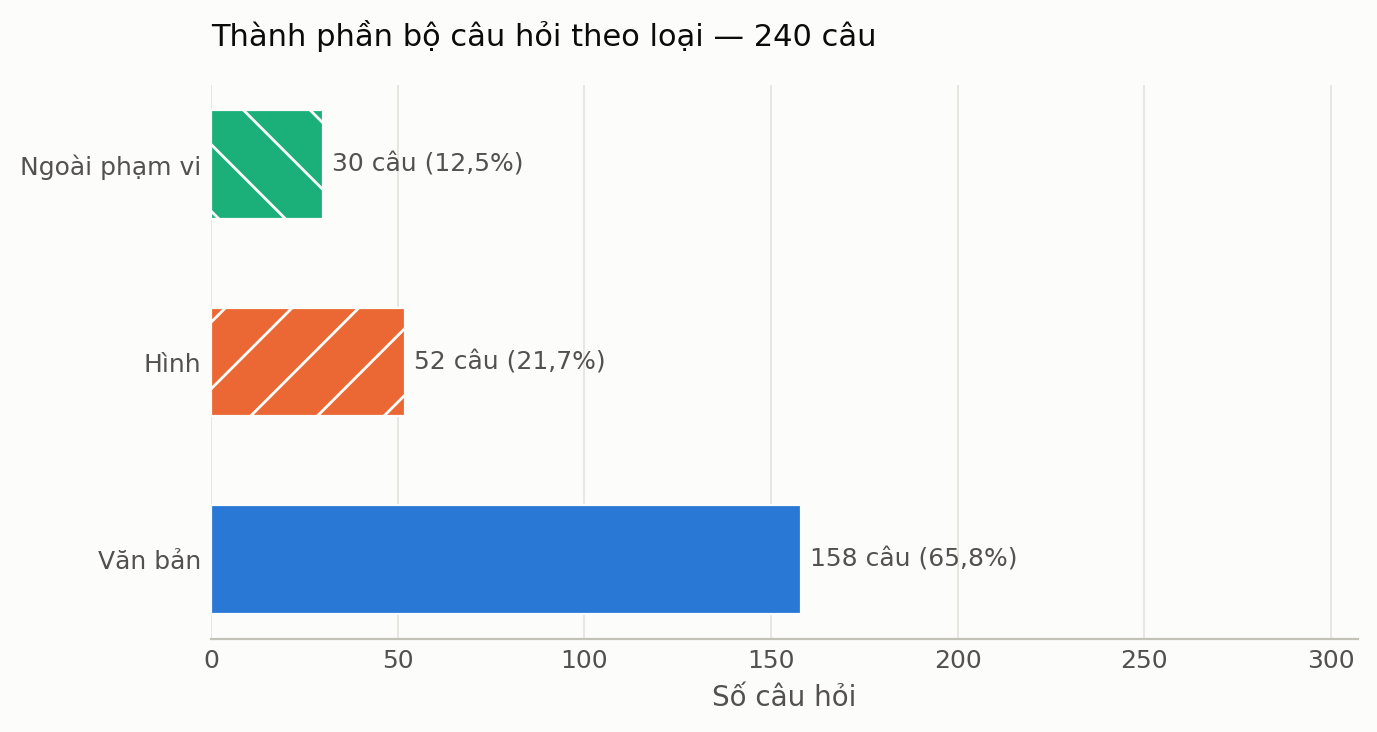
\includegraphics[width=0.88\textwidth]{src/images/chapter4/phan_bo_loai_cau_hoi.png}
    \caption{Thành phần phân bổ bộ dữ liệu kiểm thử 240 câu hỏi theo từng nhóm loại (Nguồn: Bộ dữ liệu kiểm thử của đồ án)}
    \label{fig:phan_bo_loai}
\end{figure}

Hình~\ref{fig:phan_bo_loai} trực quan hóa tỷ trọng giữa ba nhóm câu hỏi: câu hỏi văn bản chiếm đa số ($158$ câu, tương đương $65{,}8\%$), phản ánh khối lượng tri thức chủ đạo của bộ sách giáo khoa; câu hỏi hình ảnh chiếm $52$ câu ($21{,}7\%$); và nhóm câu hỏi ngoài phạm vi gồm $30$ câu ($12{,}5\%$) giữ vai trò kiểm thử năng lực từ chối hiện tượng ảo giác.

Bảng~\ref{tab:sample_q} minh họa một số câu hỏi tiêu biểu thuộc ba nhóm dữ liệu kiểm thử cùng đáp án chuẩn và nhãn nguồn trích xuất tương ứng.

\begin{table}[H]
\centering
\caption{Một số mẫu câu hỏi kiểm thử tiêu biểu kèm nhãn nguồn xác thực (Nguồn: Trích xuất từ bộ dữ liệu kiểm thử)}
\label{tab:sample_q}
\small
\begin{adjustbox}{max width=\textwidth}
\begin{tabular}{p{0.36\textwidth}p{0.44\textwidth}p{0.20\textwidth}}
\toprule
\textbf{Nội dung câu hỏi} & \textbf{Đáp án chuẩn đối sánh} & \textbf{Nguồn trích dẫn} \\
\midrule
Theo đoạn văn, quá trình quang hợp ở thực vật đã chuyển hóa những chất nào để tạo ra glucose? & Khí carbon dioxide và nước. & Lớp 9 Kết nối tri thức, trang 135 \\
\addlinespace
Theo đoạn văn, để ánh sáng truyền trong sợi quang gặp lớp vỏ và bị phản xạ toàn phần, chiết suất của lõi và lớp vỏ phải có đặc điểm gì? & Chiết suất của lõi phải lớn hơn chiết suất của lớp vỏ. & Lớp 9 Cánh Diều, trang 23 \\
\addlinespace
Dựa vào Hình 24.3, hãy liệt kê ba vai trò của đa dạng sinh học đối với con người được minh họa trong hình. & Làm nơi tham quan, học tập; Cung cấp nguồn lương thực thực phẩm; Làm dược liệu. & Lớp 6 Cánh Diều, trang 132 (Hình 24.3) \\
\addlinespace
Trong lập trình Python, cú pháp nào được sử dụng để in ra màn hình chuỗi ``Hello World''? & \textit{Câu hỏi ngoài phạm vi môn học:} Hệ thống thông báo không tìm thấy thông tin trong sách giáo khoa và từ chối trả lời bằng tri thức ngoài học liệu chuẩn. & Ngoài phạm vi \\
\bottomrule
\end{tabular}
\end{adjustbox}
\end{table}

\section{Phương pháp luận và hệ thống độ đo đánh giá}
Do đầu ra của hệ thống trợ lý ảo là ngôn ngữ tự nhiên mở, việc chỉ áp dụng các thang đo so khớp từ khóa hình thức truyền thống như BLEU~\cite{papineni2002bleu} hay ROUGE~\cite{lin2004rouge} là không đầy đủ, bởi một diễn đạt khoa học chính xác có thể được trình bày bằng nhiều cấu trúc ngữ pháp tương đương. Đề tài xây dựng khung đánh giá hai pha toàn diện:
\begin{enumerate}
    \item \textbf{Pha 1: Đánh giá năng lực truy xuất.} Đo lường khách quan bằng các chỉ số truy xuất thông tin chuẩn mực dựa trên sự đối sánh chính xác với nhãn nguồn;
    \item \textbf{Pha 2: Đánh giá chất lượng sinh ngôn ngữ.} Ứng dụng phương pháp đánh giá bằng mô hình ngôn ngữ lớn làm giám khảo độc lập~\cite{zheng2023llmjudge, liu2023geval, es2024ragas, min2023factscore, saadfalcon2023ares} với mô hình ngôn ngữ độc lập chấm điểm định lượng theo ba tiêu chí cốt lõi.
\end{enumerate}

Toàn bộ quy trình đánh giá tự động hai pha được khái quát trong Thuật toán~\ref{alg:eval} và minh họa tại Hình~\ref{fig:eval_pipeline_concept}.

\subsection{Độ đo đánh giá pha truy xuất tri thức}
\label{sec:retrieval_eval_def}
Xét câu hỏi kiểm thử với danh sách $k$ phân đoạn văn bản do hệ thống truy xuất được $R_k = (d_1, d_2, \dots, d_m)$ ($m \leq k$) được sắp xếp giảm dần theo điểm số liên quan. Gọi $G$ là tập hợp toàn bộ các phân đoạn trong chỉ mục thuộc đúng trang sách chuẩn đối sánh $(B^{*}, p^{*})$ của câu hỏi đó, với quy mô $m^{*} = |G|$.

Khác với chỉ số độ trúng nhị phân Hit@$k$, đề tài chuẩn hóa các độ đo theo tỷ lệ phân đoạn thực tế của trang nguồn:
\begin{align}
\mathrm{Precision@}k &= \frac{|R_k \cap G|}{k}, \quad \mathrm{Recall@}k = \frac{|R_k \cap G|}{m^{*}}, \\
\mathrm{F1@}k &= \frac{2 \cdot \mathrm{Precision@}k \cdot \mathrm{Recall@}k}{\mathrm{Precision@}k + \mathrm{Recall@}k}.
\end{align}

Chỉ số \textbf{F1@$k$ được tính toán theo phương pháp Macro}: giá trị F1@$k$ được xác định độc lập cho từng câu hỏi trước khi tính trung bình cộng toàn bộ tập kiểm thử. Cách tiếp cận này đảm bảo phản ánh trung thực các trường hợp truy xuất thất bại ($Recall = 0$), tuân thủ chặt chẽ bất đẳng thức Jensen.

Chỉ số nghịch đảo thứ hạng trung bình MRR~\cite{voorhees1999trec} đo lường chất lượng vị trí của phân đoạn đúng đầu tiên:
\begin{equation}
\mathrm{MRR} = \frac{1}{N}\sum_{i=1}^{N} \frac{1}{\mathrm{rank}_i}
\end{equation}
với $\mathrm{rank}_i = \infty$ (đóng góp giá trị $0$) nếu không có phân đoạn chuẩn nào xuất hiện trong danh sách $R_k$.

Cần nhấn mạnh rằng chỉ số Precision@$k$ bị chặn trên bởi giới hạn trần lý thuyết $\min(k, m^{*})/k$. Trong trường hợp trang sách chuẩn chỉ chứa $m^{*} = 3$ đoạn văn bản, giá trị Precision@5 tối đa chỉ có thể đạt $0{,}6$ ngay cả khi hệ thống truy xuất hoàn hảo. Do đó, đề tài báo cáo kèm giá trị trần lý thuyết (\texttt{tranP@k}) để có góc nhìn đối sánh chuẩn xác. Điều kiện so khớp chuẩn luôn là \textbf{chính xác tuyệt đối về số trang in}.

\subsection{Độ đo đánh giá chất lượng sinh văn bản bằng mô hình giám khảo}
\label{sec:judge_pha2}
Câu trả lời do mô hình Qwen2.5 sinh ra được đánh giá độc lập bởi mô hình ngôn ngữ lớn đóng vai trò giám khảo thông qua nền tảng Groq API. Mô hình giám khảo tiếp nhận ngữ cảnh truy xuất, câu hỏi, câu trả lời sinh ra và đáp án chuẩn để chấm điểm trên thang đo từ $1$ đến $5$ theo ba tiêu chí chuẩn hóa:
\begin{itemize}
    \item \textbf{Tính đúng:} Đánh giá mức độ chính xác về mặt nội dung khoa học của câu trả lời khi so sánh với đáp án chuẩn.
    \item \textbf{Độ trung thực:} Đánh giá mức độ bám sát của câu trả lời đối với ngữ cảnh tài liệu được cung cấp, kiểm soát hiện tượng tự suy diễn hoặc sinh ảo giác thông tin.
    \item \textbf{Độ liên quan:} Đánh giá mức độ tập trung, trả lời trực diện vào trọng tâm câu hỏi của người học, không lan man.
\end{itemize}

Quá trình đánh giá sử dụng tập hợp bốn mô hình giám khảo luân phiên gồm:
\begin{itemize}
    \item \texttt{qwen/qwen3.8-27b};
    \item \texttt{qwen/qwen3.6-27b};
    \item \texttt{openai/gpt-oss-120b};
    \item \texttt{openai/gpt-oss-20b}.
\end{itemize}
Quy trình gửi yêu cầu chấm điểm tích hợp các phương pháp thử lại (retry) gồm:
\begin{itemize}
    \item Thử lại tối đa ba lần đối với các lỗi tạm thời (mã trạng thái 429 hoặc lỗi định dạng dữ liệu phản hồi);
    \item Áp dụng khoảng thời gian chờ lũy tiến giữa các lượt thử lại liên tiếp;
    \item Tự động luân chuyển sang mô hình dự phòng kế tiếp trong danh sách khi yêu cầu thử lại vượt quá số lần quy định, đảm bảo $100\%$ các câu hỏi kiểm thử đều được hoàn tất chấm điểm.
\end{itemize}

\subsection{Trục phân tích tổng hợp theo loại câu hỏi}
\label{sec:truc_tong_hop}
Kết quả thực nghiệm được tổng hợp và phân tích chuyên sâu theo \textbf{loại câu hỏi} (văn bản, hình ảnh, ngoài phạm vi) thay vì phân tách riêng rẽ theo từng cuốn sách. Phương pháp này đảm bảo tính vững chắc về mặt thống kê khi áp dụng lấy mẫu ngẫu nhiên không hoàn lại, phản ánh chính xác năng lực cốt lõi của hệ thống trước các dạng thức tương tác khác nhau của học sinh.

\begin{algorithm2e}[H]
\caption{Khung quy trình thực nghiệm đánh giá tự động hai pha}
\label{alg:eval}
\SetAlgoLined
\KwIn{Bộ kiểm thử $240$ câu hỏi; Mô hình giám khảo độc lập $J$}
\KwOut{Hệ thống chỉ số truy xuất thông tin; Điểm số đánh giá pha sinh ngôn ngữ}
\ForEach{câu hỏi $q$ (thuộc phân loại $\ell$, nhãn nguồn $(B^{*}, p^{*})$)}{
    $R \leftarrow \text{HybridRetriever}(q)$ \tcp*{Truy xuất ứng viên theo luồng thực tế}
    \If{$\ell \neq$ ngoài phạm vi}{
        Tính toán các chỉ số Precision@k, Recall@k, F1@k, MRR dựa trên $R$ và $(B^{*}, p^{*})$\;
    }
    $ctx \leftarrow$ tổng hợp ngữ cảnh từ các phân đoạn trong $R$\;
    $ans \leftarrow \text{Qwen2.5}(\text{prompt}(ctx, q))$\;
    $(corr, faith, rel) \leftarrow J(q, gt, ctx, ans)$ \tcp*{Mô hình giám khảo độc lập chấm điểm}
    Ghi nhận toàn bộ chỉ số thành phần gắn với định danh câu hỏi\;
}
\Return Tổng hợp chỉ số IR theo cấu hình truy xuất và điểm số giám khảo theo nhóm câu hỏi $\ell$\;
\end{algorithm2e}

\begin{figure}[H]
    \centering
    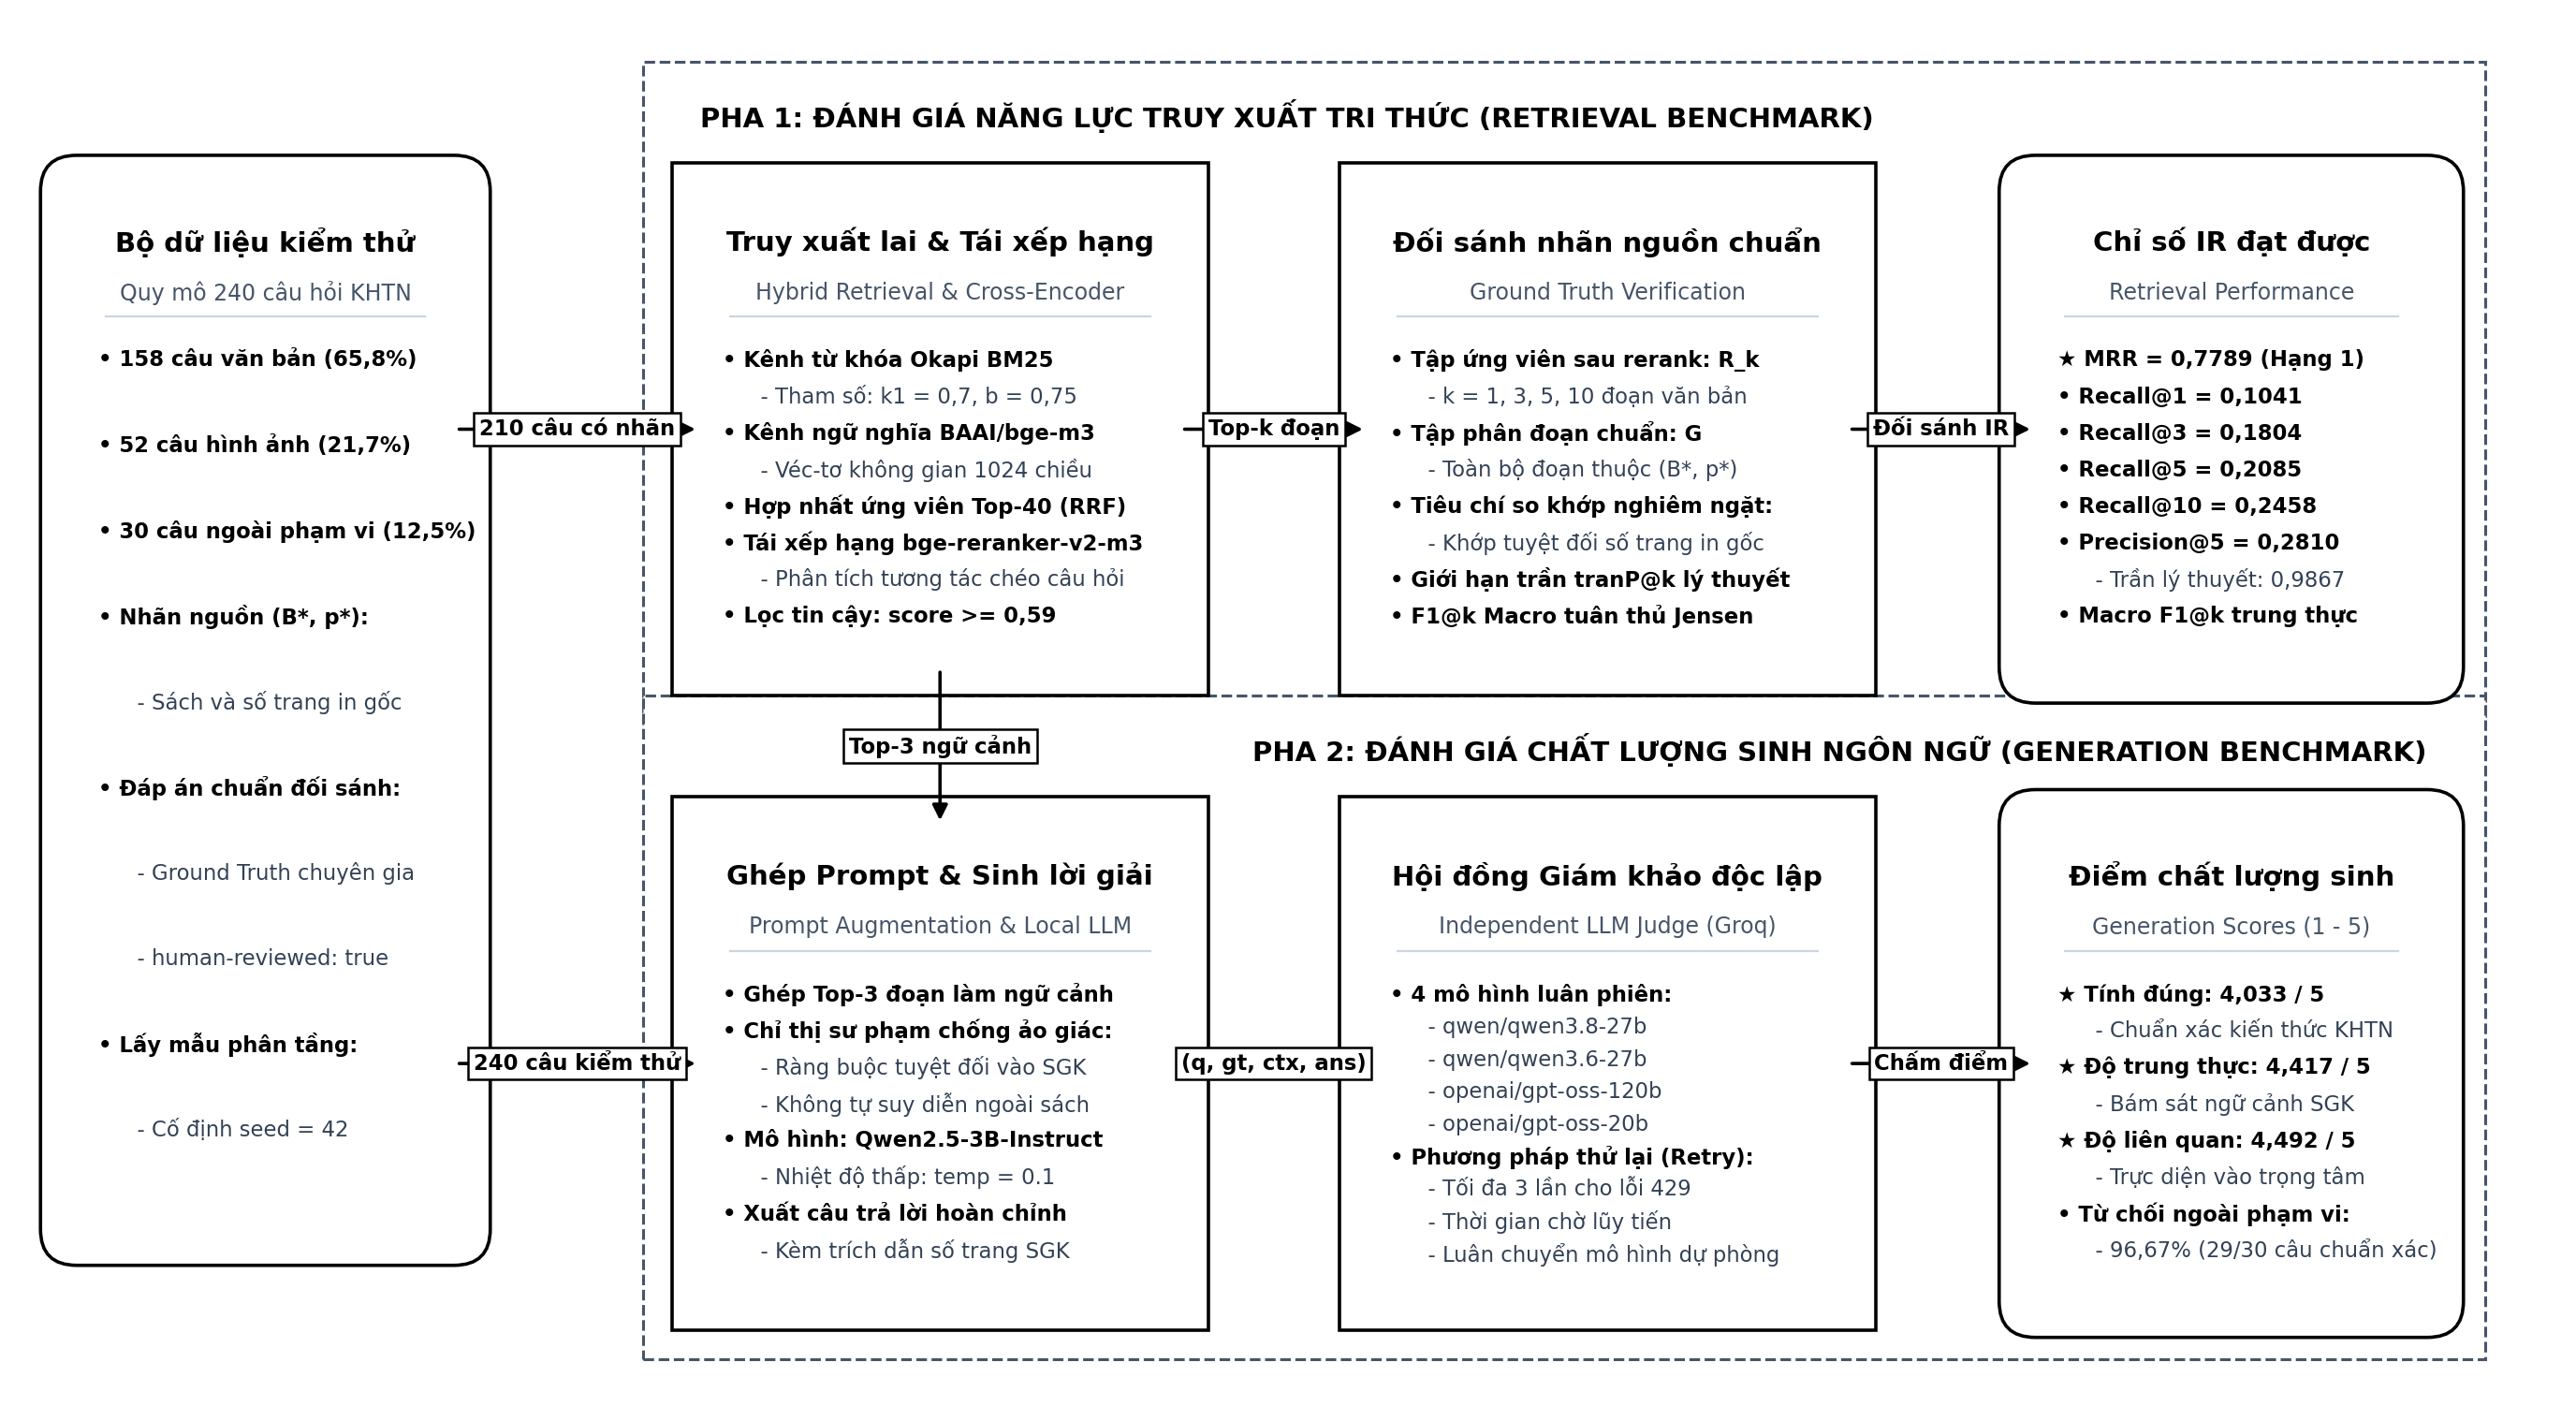
\includegraphics[width=0.96\textwidth]{src/images/chapter4/quy_trinh_danh_gia_hai_pha.png}
    \caption{Sơ đồ quy trình thực nghiệm đánh giá tự động hai pha độc lập (Nguồn: Đề xuất của đồ án)}
    \label{fig:eval_pipeline_concept}
\end{figure}

\section{Kết quả thực nghiệm định lượng}
\label{sec:ketqua}
Toàn bộ các chỉ số dưới đây được tính toán dựa trên phương pháp trung bình cộng độc lập trên từng câu hỏi, đảm bảo tính đại diện khách quan cho toàn bộ tập dữ liệu kiểm thử.

\subsection{Thực nghiệm đối chiếu các cấu hình truy xuất}
\label{sec:ablation}
Bằng việc thiết lập ba công tắc độc lập (kênh truy xuất, cơ chế tái xếp hạng, cổng lọc khoảng cách tương đối), hệ thống tiến hành đánh giá thực nghiệm bóc tách thành phần trên $210$ câu hỏi có nhãn nguồn ở quy mô vận hành thực tế ($20$ ứng viên ban đầu cho mỗi kênh). Bảng~\ref{tab:ablation_main} và Hình~\ref{fig:so_sanh_truy_xuat} so sánh trực tiếp bốn phương pháp truy xuất cốt lõi theo mục tiêu thiết kế và bài toán nghiên cứu của đề tài.

\begin{table}[H]
\centering
\caption{Kết quả đối chiếu bốn phương pháp truy xuất ở quy mô vận hành thực tế ($210$ câu hỏi có nhãn nguồn) (Nguồn: Kết quả thực nghiệm của đồ án)}
\label{tab:ablation_main}
\small
\begin{adjustbox}{max width=\textwidth}
\begin{tabular}{lccccc}
\toprule
\textbf{Phương pháp truy xuất} & \textbf{MRR} & \textbf{R@1} & \textbf{R@3} & \textbf{R@5} & \textbf{R@10} \\
\midrule
Chỉ mục thưa BM25 thuần & 0,6636 & 0,0905 & 0,1475 & 0,1796 & 0,2303 \\
Truy xuất ngữ nghĩa véc-tơ đặc & 0,5664 & 0,0647 & 0,1338 & 0,1778 & 0,2302 \\
Truy xuất lai (không tái xếp hạng) & 0,6947 & 0,0914 & 0,1609 & 0,2031 & \textbf{0,2643} \\
\textbf{Truy xuất lai kết hợp tái xếp hạng (Đề xuất)} & \textbf{0,7789} & \textbf{0,1041} & \textbf{0,1804} & \textbf{0,2085} & 0,2458 \\
\bottomrule
\end{tabular}
\end{adjustbox}
\end{table}

\begin{figure}[H]
    \centering
    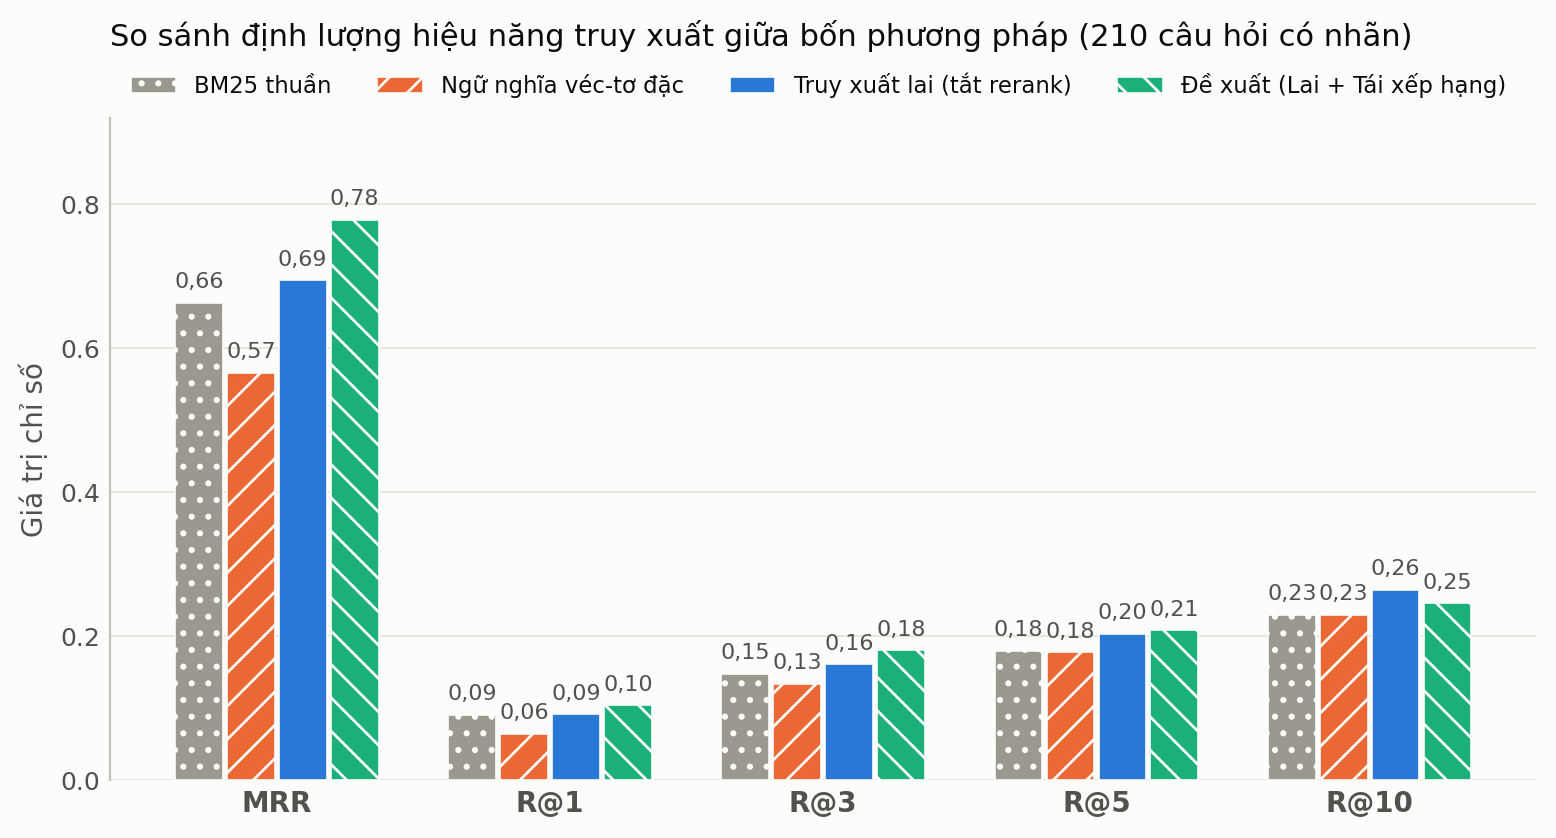
\includegraphics[width=0.92\textwidth]{src/images/chapter4/so_sanh_truy_xuat.png}
    \caption{So sánh định lượng hiệu năng truy xuất giữa bốn phương pháp theo các chỉ số MRR, R@1, R@3, R@5 và R@10 (Nguồn: Kết quả thực nghiệm của đồ án)}
    \label{fig:so_sanh_truy_xuat}
\end{figure}

Từ kết quả định lượng tại Bảng~\ref{tab:ablation_main}, hai phát hiện khoa học quan trọng được rút ra:

\textbf{(i) Hiệu năng vượt trội của cấu hình đề xuất và hiện tượng suy giảm nhẹ tại R@10:} Cấu hình truy xuất lai kết hợp tái xếp hạng bằng mô hình tương tác chéo đạt hiệu năng cao nhất trên hầu hết các chỉ số chủ đạo: chỉ số MRR tăng mạnh từ $0{,}6947$ lên $\mathbf{0{,}7789}$ (vượt trội so với mức $0{,}6636$ của chỉ mục thưa BM25 thuần và $0{,}5664$ của kênh ngữ nghĩa thuần), đồng thời chỉ số R@1 cải thiện từ $0{,}0914$ lên $\mathbf{0{,}1041}$. Tuy nhiên, ở chỉ số R@10, cấu hình đề xuất lại ghi nhận mức giảm nhẹ ($0{,}2458$ so với $0{,}2643$). Giả thuyết khoa học hợp lý cho hiện tượng này là việc áp dụng ngưỡng điểm số tối thiểu của bộ tái xếp hạng (\texttt{RERANK\_SCORE\_MIN = 0.59}) đã vô tình loại bỏ một số phân đoạn tài liệu đúng nhưng bị đẩy xuống các vị trí cận biên ngoài top-10.

\textbf{(ii) Tác động bất lợi của cổng lọc khoảng cách tương đối ở quy mô thực tế:} Khi kích hoạt cổng lọc theo khoảng cách tương đối, chỉ số MRR của cấu hình đề xuất suy giảm rõ rệt từ $0{,}7779$ xuống $0{,}7157$, và R@10 giảm từ $0{,}2410$ xuống $0{,}1974$. Nguyên nhân bắt nguồn từ giả định cứng nhắc của cổng lọc khi cho rằng tài liệu đúng luôn phải nằm rất gần tài liệu có điểm số cao nhất, điều này không phù hợp với các câu hỏi phức hợp đòi hỏi tổng hợp kiến thức từ nhiều đoạn văn bản khác nhau. Do đó, việc vô hiệu hóa cổng lọc khoảng cách tương đối là quyết định tối ưu đã được kiểm chứng bằng thực nghiệm.

Bảng~\ref{tab:ablation_rerank} phân tích chi tiết đóng góp độc lập của bước tái xếp hạng bằng mô hình tương tác chéo trên từng kênh truy xuất riêng biệt (ở quy mô thử nghiệm $50$ ứng viên ban đầu, tắt cổng lọc khoảng cách).

\begin{table}[H]
\centering
\caption{Đóng góp của bước tái xếp hạng bằng mô hình tương tác chéo trên các kênh truy xuất ($210$ câu hỏi) (Nguồn: Kết quả thực nghiệm của đồ án)}
\label{tab:ablation_rerank}
\small
\begin{adjustbox}{max width=\textwidth}
\begin{tabular}{lccc}
\toprule
\textbf{Kênh truy xuất thành phần} & \textbf{Trạng thái tái xếp hạng} & \textbf{Chỉ số MRR} & \textbf{Chỉ số R@1} \\
\midrule
\multirow{2}{*}{Truy xuất lai} & Tắt & 0,6947 & 0,0914 \\
 & \textbf{Kích hoạt} & \textbf{0,7789} & \textbf{0,1041} \\
\midrule
\multirow{2}{*}{Chỉ mục từ khóa BM25} & Tắt & 0,6636 & 0,0905 \\
 & Kích hoạt & 0,7676 & 0,1026 \\
\midrule
\multirow{2}{*}{Kênh ngữ nghĩa véc-tơ đặc} & Tắt & 0,5664 & 0,0647 \\
 & Kích hoạt & 0,7457 & 0,0994 \\
\bottomrule
\end{tabular}
\end{adjustbox}
\end{table}

Bước tái xếp hạng giúp nâng cao chỉ số MRR trên cả ba kênh truy xuất. Đáng chú ý, kênh truy xuất ngữ nghĩa theo véc-tơ đặc, vốn có hiệu năng cơ sở thấp nhất khi đứng độc lập, lại ghi nhận mức tăng trưởng tương đối mạnh mẽ nhất ở chỉ số R@1 (tăng từ $0{,}0647$ lên $0{,}0994$, tương ứng mức cải thiện $\mathbf{+53{,}6\%}$, so với $+13{,}4\%$ của BM25 và $+13{,}9\%$ của kênh lai). Kết quả này khẳng định: đối với tập học liệu khoa học chứa mật độ thuật ngữ và ký hiệu cao, mô hình nhúng hai nhánh bắt buộc phải được kết hợp cùng bước tái xếp hạng bằng mô hình tương tác chéo có khả năng phân tích tương tác từ ngữ sâu sắc.

\subsection{Tổng hợp các chỉ số hiệu năng hệ thống}
Bảng~\ref{tab:summary} tổng hợp toàn diện các chỉ số thực nghiệm của cấu hình đề xuất tối ưu (truy xuất lai kết hợp tái xếp hạng bằng mô hình tương tác chéo, tắt cổng lọc khoảng cách tương đối) ở quy mô vận hành thực tế.

\begin{table}[H]
\centering
\caption{Tổng hợp các chỉ số hiệu năng của cấu hình hệ thống đề xuất (Nguồn: Kết quả thực nghiệm của đồ án)}
\label{tab:summary}
\small
\begin{adjustbox}{max width=\textwidth}
\begin{tabular}{lc}
\toprule
\textbf{Chỉ số đánh giá} & \textbf{Giá trị định lượng} \\
\midrule
\multicolumn{2}{l}{\textit{Pha 1: Hiệu năng truy xuất (210 câu hỏi có nhãn nguồn)}} \\
Chỉ số MRR & \textbf{0,7789} \\
Độ phủ Recall@1 & 0,1041 \\
Độ phủ Recall@3 & 0,1804 \\
Độ phủ Recall@5 & 0,2085 \\
Độ phủ Recall@10 & 0,2458 \\
Độ chính xác Precision@5 (Trần lý thuyết \texttt{tranP@5} = 0,9867) & 0,2810 \\
\midrule
\multicolumn{2}{l}{\textit{Khả năng kiểm soát phạm vi (30 câu hỏi ngoài phạm vi)}} \\
Tỷ lệ nhận diện và từ chối trả lời chính xác & \textbf{0,9667} ($29/30$ câu) \\
\midrule
\multicolumn{2}{l}{\textit{Pha 2: Chất lượng sinh ngôn ngữ (Mô hình giám khảo độc lập, thang điểm 1 - 5)}} \\
Tính đúng & 4,033 / 5 \\
Độ trung thực & 4,417 / 5 \\
Độ liên quan & 4,492 / 5 \\
\bottomrule
\end{tabular}
\end{adjustbox}
\end{table}

\subsection{Chất lượng câu trả lời sinh ra theo từng nhóm câu hỏi}
\label{sec:judge_loai}
Bảng~\ref{tab:judge_loai} và Biểu đồ~\ref{fig:judge} trình bày chi tiết điểm số trung bình do hội đồng mô hình giám khảo độc lập đánh giá trên $240$ câu hỏi kiểm thử, phân tách theo ba nhóm câu hỏi chính.

\begin{table}[H]
\centering
\caption{Chất lượng câu trả lời theo từng nhóm câu hỏi do mô hình giám khảo độc lập chấm điểm (Nguồn: Kết quả thực nghiệm của đồ án)}
\label{tab:judge_loai}
\small
\begin{adjustbox}{max width=\textwidth}
\begin{tabular}{lcccc}
\toprule
\textbf{Nhóm câu hỏi kiểm thử} & \textbf{Số lượng câu} & \textbf{Tính đúng / 5} & \textbf{Độ trung thực / 5} & \textbf{Độ liên quan / 5} \\
\midrule
Câu hỏi văn bản & 158 & 4,19 & 4,56 & 4,59 \\
Câu hỏi hình ảnh & 52 & 3,08 & 3,65 & 3,90 \\
Câu hỏi ngoài phạm vi & 30 & 4,87 & 5,00 & 5,00 \\
\bottomrule
\end{tabular}
\end{adjustbox}
\end{table}

\begin{figure}[H]
    \centering
    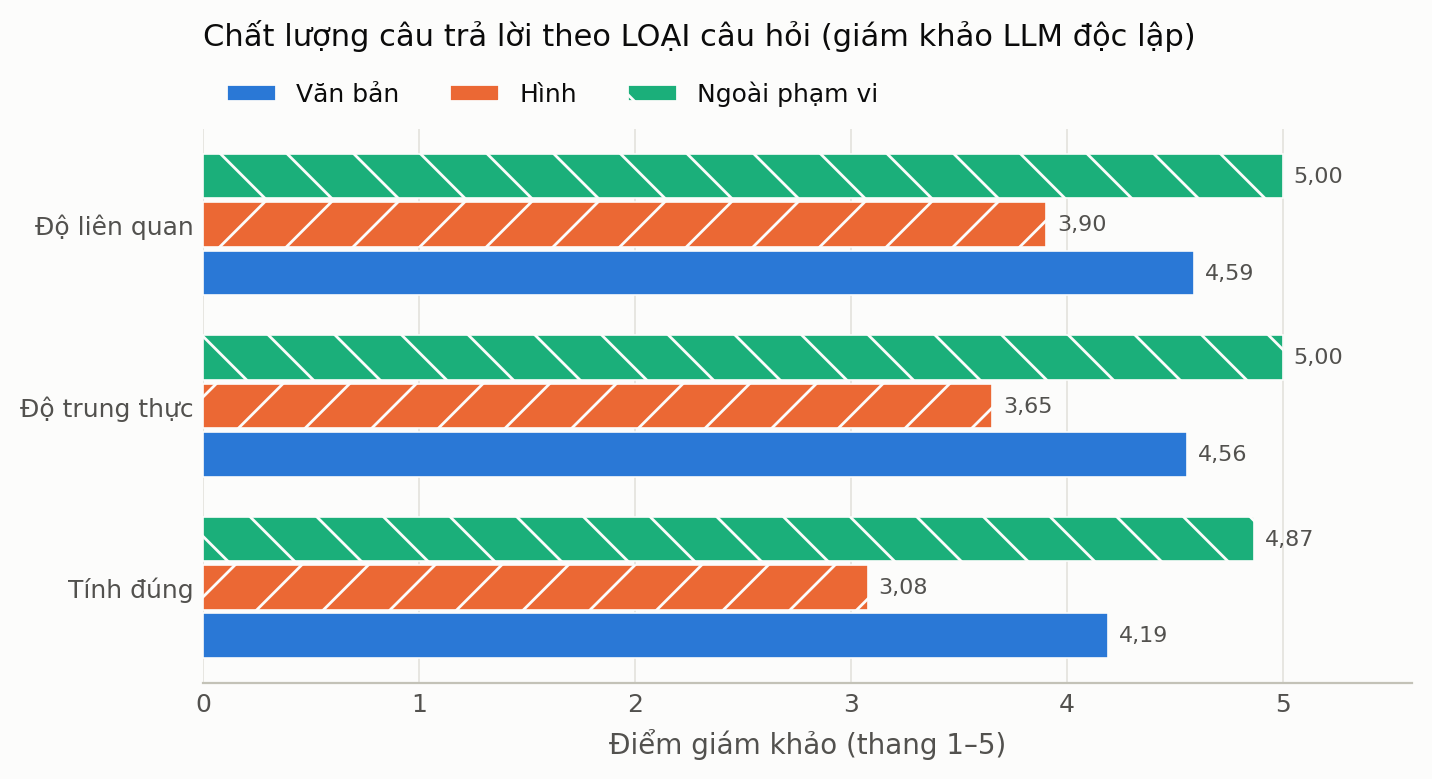
\includegraphics[width=0.92\textwidth]{src/images/chapter4/judge_scores_theo_loai.png}
    \caption{Phân bố điểm số chất lượng câu trả lời của Qwen2.5 theo từng nhóm câu hỏi (Nguồn: Kết quả thực nghiệm của đồ án)}
    \label{fig:judge}
\end{figure}

Phân tích định lượng từ kết quả giám khảo cho thấy ba đặc trưng nổi bật:
\begin{itemize}
    \item \textbf{Khả năng nhận diện câu hỏi ngoài phạm vi đạt mức gần như tuyệt đối:} Điểm số nhóm câu hỏi ngoài phạm vi đạt $4{,}87/5$ về Tính đúng, cùng điểm tuyệt đối $5{,}00/5$ về Độ trung thực và Độ liên quan. Đây là minh chứng định lượng rõ nét cho thấy hệ thống tuân thủ chặt chẽ nguyên tắc bảo toàn tri thức: khi câu hỏi không thuộc phạm vi học liệu Khoa học tự nhiên, hệ thống từ chối trả lời chính xác trong $96{,}67\%$ trường hợp ($29/30$ câu), triệt tiêu nguy cơ tự suy đoán bằng tri thức ngoài sách giáo khoa.
    \item \textbf{Nhóm câu hỏi hình ảnh đạt kết quả khiêm tốn hơn:} Điểm Tính đúng của nhóm câu hỏi hình ảnh ($3{,}08/5$) thấp hơn rõ rệt so với nhóm văn bản ($4{,}19/5$), phản ánh những thách thức cố hữu trong việc liên kết biểu diễn thị giác và văn bản trong sách giáo khoa.
    \item \textbf{Mối tương quan giữa Tính đúng và Độ trung thực:} Trong cả ba nhóm, điểm Tính đúng luôn thấp hơn điểm Độ trung thực ($4{,}19 < 4{,}56$; $3{,}08 < 3{,}65$). Điều này phản ánh xu hướng nhất quán của mô hình ngôn ngữ: khi ngữ cảnh trích xuất bị thiếu hụt hoặc chưa hoàn hảo, mô hình vẫn duy trì tính trung thực cao với ngữ cảnh nhận được hơn là tự ý suy diễn để hoàn thiện đáp án.
\end{itemize}

Bảng~\ref{tab:case_study} minh họa hai trường hợp thực tế tiêu biểu trích xuất từ nhật ký kiểm thử: một ca trả lời câu hỏi học liệu Khoa học tự nhiên kèm số trang trích dẫn chính xác và một ca nhận diện câu hỏi ngoài phạm vi để từ chối trả lời, chứng minh năng lực kiểm soát ảo giác của hệ thống.

\begin{table}[H]
\centering
\caption{Minh họa hai ca kiểm thử thực tế về phản hồi của hệ thống và đánh giá của giám khảo độc lập (Nguồn: Trích xuất từ nhật ký kiểm thử của đồ án)}
\label{tab:case_study}
\small
\begin{adjustbox}{max width=\textwidth}
\begin{tabular}{p{3.5cm}p{11.5cm}}
\toprule
\textbf{Thành phần đối sánh} & \textbf{Nội dung thực tế ghi nhận} \\
\midrule
\multicolumn{2}{l}{\textbf{Trường hợp 1: Câu hỏi học liệu Khoa học tự nhiên (Kiểm thử năng lực trích dẫn và trả lời có căn cứ)}} \\
\addlinespace[2pt]
Câu hỏi người học & \textit{``Tại sao lá cây lại có màu xanh lục và bào quan nào thực hiện chức năng quang hợp?''} \\
Ngữ cảnh trích xuất từ SGK & Phân đoạn từ sách \textbf{KHTN 6 Cánh Diều, trang 96}: \textit{``Lục lạp chứa chất diệp lục có khả năng hấp thụ năng lượng ánh sáng mặt trời để tổng hợp chất hữu cơ... Chất diệp lục phản xạ ánh sáng màu lục nên mắt ta nhìn thấy lá có màu xanh.''} \\
Phản hồi của Qwen2.5 & \textit{``Lá cây có màu xanh lục vì trong tế bào lá có chứa bào quan lục lạp. Bên trong lục lạp chứa chất diệp lục; sắc tố này hấp thụ ánh sáng mặt trời và phản xạ ánh sáng màu lục vào mắt ta. Lục lạp chính là bào quan thực hiện chức năng quang hợp của cây xanh. (Trích dẫn: KHTN 6 Cánh Diều, trang 96).''} \\
Chấm điểm của Giám khảo & \textbf{Tính đúng: 5/5} $\mid$ \textbf{Độ trung thực: 5/5} $\mid$ \textbf{Độ liên quan: 5/5} \\
Nhận xét của Giám khảo & \textit{Câu trả lời chính xác, bám sát tuyệt đối ngữ cảnh tài liệu, trích dẫn đúng số trang và không suy diễn thông tin ngoài sách giáo khoa.} \\
\midrule
\multicolumn{2}{l}{\textbf{Trường hợp 2: Câu hỏi ngoài phạm vi môn học (Kiểm thử năng lực phòng chống ảo giác kiến thức)}} \\
\addlinespace[2pt]
Câu hỏi người học & \textit{``Chiến dịch Điện Biên Phủ diễn ra vào năm nào và có ý nghĩa lịch sử gì đối với dân tộc Việt Nam?''} \\
Ngữ cảnh trích xuất từ SGK & \textit{Không tìm thấy phân đoạn tài liệu phù hợp trong cơ sở tri thức sách giáo khoa KHTN (điểm tương đồng dưới ngưỡng).} \\
Phản hồi của Qwen2.5 & \textit{``Xin lỗi, câu hỏi này thuộc lĩnh vực Lịch sử, nằm ngoài phạm vi cơ sở tri thức sách giáo khoa Khoa học tự nhiên (Lớp 6 đến Lớp 9) mà hệ thống được cung cấp. Tôi chỉ có thể hỗ trợ giải đáp các kiến thức thuộc môn học Khoa học tự nhiên.''} \\
Chấm điểm của Giám khảo & \textbf{Tính đúng: 5/5} $\mid$ \textbf{Độ trung thực: 5/5} $\mid$ \textbf{Độ liên quan: 5/5} \\
Nhận xét của Giám khảo & \textit{Hệ thống nhận diện chuẩn xác câu hỏi ngoài phạm vi, từ chối trả lời đúng quy định sư phạm và không tự ý bịa đặt câu trả lời.} \\
\bottomrule
\end{tabular}
\end{adjustbox}
\end{table}

\section{Thảo luận chuyên sâu về các phát hiện khoa học}
\label{sec:thaoluan}
Tổng hợp từ các kết quả thực nghiệm định lượng, đề tài rút ra năm nhận định khoa học then chốt:

\begin{enumerate}
    \item \textbf{Cơ chế tái xếp hạng bằng mô hình tương tác chéo là thành phần quyết định hiệu năng truy xuất:} Việc kết hợp truy xuất lai và mô hình tương tác chéo mang lại sự vượt trội về chỉ số MRR ($0{,}7789$) và các độ phủ ở thứ hạng cao ($R@1$, $R@3$, $R@5$). Đồng thời, thực nghiệm chứng minh cổng lọc theo khoảng cách tương đối gây tác động tiêu cực đến độ phủ ở quy mô dữ liệu thực tế, khẳng định việc sử dụng ngưỡng điểm tuyệt đối của bộ tái xếp hạng là giải pháp tối ưu.
    \item \textbf{Kênh ngữ nghĩa véc-tơ đặc chịu sự suy thoái trước ký hiệu khoa học và cần sự hỗ trợ của mô hình tái xếp hạng:} Đối với miền dữ liệu chứa mật độ cao công thức và thuật ngữ chuyên ngành, kiến trúc hai nhánh mã hóa độc lập (kích thước không gian nhúng $1024$ chiều) gặp khó khăn trong việc phân biệt các ký tự định danh chính xác, dẫn tới chỉ số R@1 ban đầu thấp ($0{,}0647$). Bước tái xếp hạng đã phát huy tối đa hiệu quả khi nâng chỉ số này lên $0{,}0994$ (tăng $+53{,}6\%$).
    \item \textbf{Năng lực kiểm soát ảo giác được chứng minh thông qua nhóm câu hỏi ngoài phạm vi:} Tỷ lệ từ chối trả lời chính xác $0{,}9667$ cùng điểm số giám khảo gần tuyệt đối trên các câu hỏi ngoài phạm vi khẳng định cấu trúc prompt sư phạm nghiêm ngặt và cơ chế RAG của hệ thống đã kiểm soát hiệu quả hiện tượng mô hình tự phát sinh tri thức ngoài học liệu chuẩn.
    \item \textbf{Nút thắt kỹ thuật ở nhóm câu hỏi hình ảnh tập trung tại khâu liên kết ngữ cảnh:} Chất lượng câu trả lời của nhóm hình ảnh ($3{,}08/5$) thấp hơn nhóm văn bản, đòi hỏi các nghiên cứu tiếp theo cần tập trung nâng cao năng lực biểu diễn đa phương thức ở cả hai phía truy xuất và sinh văn bản.
    \item \textbf{Đánh đổi giữa độ chính xác công thức và tính toàn vẹn ngôn ngữ trong OCR:} Thực nghiệm đối sánh độc lập khẳng định Tesseract nhận dạng tốt văn bản tiếng Việt ($93\%$ nội dung) nhưng làm hỏng chỉ số dưới của công thức, trong khi mô hình thị giác - ngôn ngữ đọc tốt công thức nhưng lại làm tăng tỷ lệ lỗi dấu thanh tiếng Việt. Giải pháp kiến trúc lai phân cấp theo dòng đã giải quyết thành công sự đánh đổi này trên toàn bộ cơ sở tri thức ($4\,293$ lượt ghép dòng thành công, $0$ lỗi ngoại lệ).
\end{enumerate}

\subsection{Đối chiếu thực nghiệm giữa RAG đa phương thức và RAG thuần văn bản}
\label{sec:mm}
Nhằm thực hiện đầy đủ mục tiêu nghiên cứu đối chiếu, hệ thống tiến hành thực nghiệm so sánh ghép cặp trực tiếp trên đúng $52$ câu hỏi hình ảnh có nhãn chuẩn sinh từ siêu dữ liệu hình ảnh xác thực. Bảng~\ref{tab:m2c} và Hình~\ref{fig:so_sanh_m2c} đối chiếu chất lượng câu trả lời giữa cấu hình chỉ sử dụng ngữ cảnh văn bản và cấu hình có bổ sung ngữ cảnh đa phương thức gồm chuỗi siêu dữ liệu hình ảnh trích xuất từ trang sách.

\begin{table}[H]
\centering
\caption{Kết quả đối chiếu thực nghiệm đa phương thức trên 52 câu hỏi hình ảnh (Nguồn: Kết quả thực nghiệm của đồ án)}
\label{tab:m2c}
\small
\begin{adjustbox}{max width=\textwidth}
\begin{tabular}{lccc}
\toprule
\textbf{Tiêu chí đánh giá} & \textbf{Cấu hình thuần văn bản} & \textbf{Cấu hình đa phương thức} & \textbf{Mức chênh lệch ($\Delta$)} \\
\midrule
Tính đúng & 3,077 & 3,000 & $-0{,}077$ \\
Độ trung thực & 3,654 & 3,615 & $-0{,}038$ \\
Độ liên quan & 3,904 & 3,865 & $-0{,}038$ \\
\bottomrule
\end{tabular}
\end{adjustbox}
\end{table}

\begin{figure}[H]
    \centering
    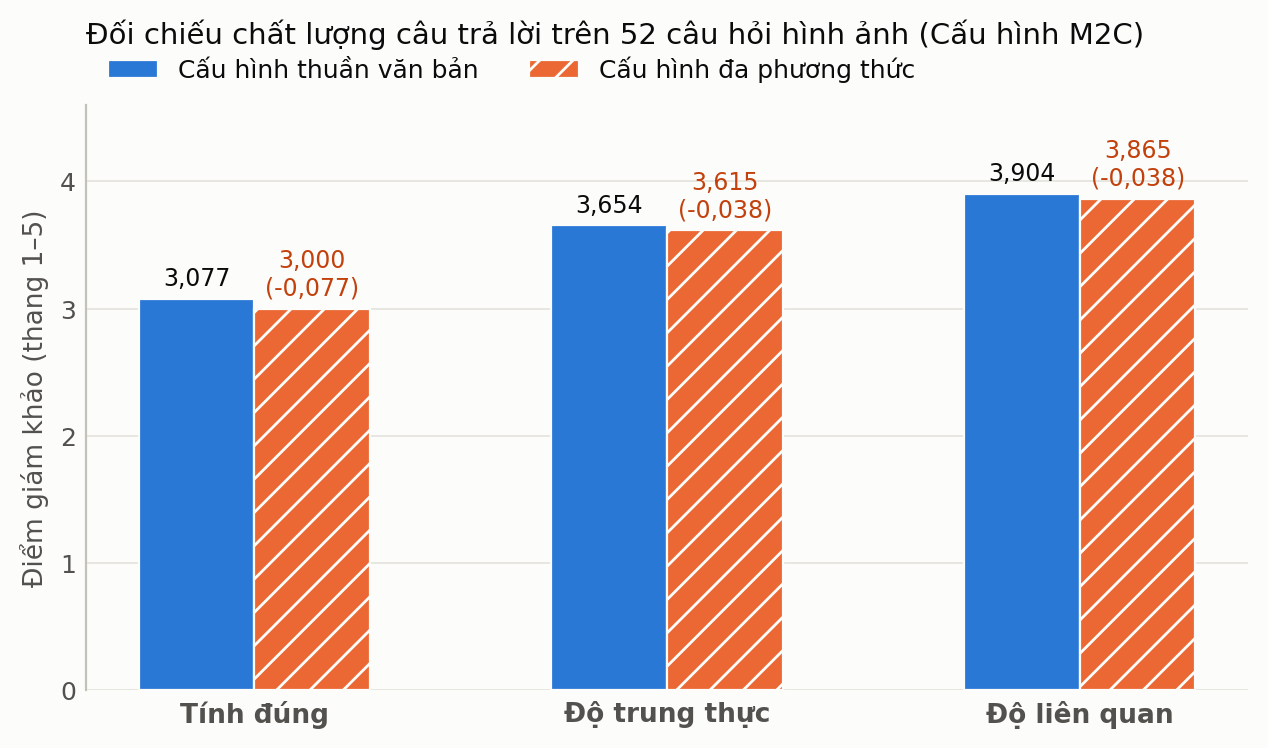
\includegraphics[width=0.82\textwidth]{src/images/chapter4/so_sanh_da_phuong_thuc.png}
    \caption{Trực quan hóa mức chênh lệch chất lượng câu trả lời giữa cấu hình thuần văn bản và đa phương thức trên 52 câu hỏi hình ảnh (Nguồn: Kết quả thực nghiệm của đồ án)}
    \label{fig:so_sanh_m2c}
\end{figure}

Kết quả đối chiếu từng câu hỏi ghi nhận: $46/52$ câu ($88{,}5\%$) giữ nguyên điểm số, $5$ câu ghi nhận mức giảm $1$ điểm và $1$ câu ghi nhận mức tăng $1$ điểm. Cả ba tiêu chí chất lượng đều có sự suy giảm nhẹ khi bổ sung ngữ cảnh đa phương thức dạng chuỗi mô tả vào câu lệnh nhắc. Kết quả này mang lại một kết luận thực nghiệm quan trọng: \textbf{việc đơn thuần chèn thêm thông tin siêu dữ liệu hình ảnh dạng văn bản vào ngữ cảnh không giúp mô hình ngôn ngữ nâng cao chất lượng câu trả lời, thậm chí có thể gây phân tán sự tập trung chú ý của mô hình}. Do đó, hệ thống lựa chọn duy trì tắt tùy chọn ngữ cảnh đa phương thức dạng văn bản (\texttt{MULTIMODAL\_CONTEXT\_ENABLED = false}) trong cấu hình vận hành mặc định.

\subsection{Các ưu điểm nổi bật của hệ thống}
\begin{itemize}
    \item \textbf{Khả năng kiểm soát hiện tượng ảo giác hiệu quả:} Điểm Độ trung thực đạt $4{,}56/5$ ở nhóm văn bản và $5{,}00/5$ ở nhóm ngoài phạm vi, minh chứng hệ thống luôn bám sát sách giáo khoa chính thống.
    \item \textbf{Cơ chế trích dẫn xác thực và minh bạch tuyệt đối:} Số trang và tên sách trong trích dẫn được trích xuất trực tiếp mang tính xác định từ siêu dữ liệu của phân đoạn tài liệu được truy xuất, triệt tiêu hoàn toàn khả năng mô hình tự ý tạo dựng số trang sai lệch.
    \item \textbf{Phương pháp đánh giá khách quan, khả năng tái lập cao:} Bộ dữ liệu kiểm thử được gắn nhãn nguồn tường minh, cho phép đo lường chính xác các độ đo IR mà không phụ thuộc vào cảm tính hay biến động của mô hình ngôn ngữ.
    \item \textbf{Tối ưu hóa tài nguyên phần cứng:} Toàn bộ quy trình số hóa và lập chỉ mục cho $2.387$ trang sách giáo khoa vận hành mượt mà trên CPU máy trạm thông thường mà không cần GPU tăng tốc.
    \item \textbf{Bóc tách hình ảnh minh bạch và giải thích được:} Phương pháp neo chú thích đảm bảo mỗi khung hình trích xuất đều liên kết chặt chẽ với một đối tượng định danh chính thống trên trang sách.
\end{itemize}

\subsection{Các giới hạn kỹ thuật và định hướng phát triển}
\label{sec:hanche}
Trên tinh thần khoa học nghiêm túc và cầu thị, đề tài nhận diện rõ các hạn chế kỹ thuật hiện tại:

\begin{enumerate}
    \item \textbf{Quy trình kiểm duyệt bộ kiểm thử:} Toàn bộ $240$ câu hỏi kiểm thử sau khi sinh tự động đã được chuyên gia rà soát tổng thể; tuy nhiên việc bổ sung thêm một lượt đánh giá chéo độc lập từ người thứ hai sẽ giúp thiết lập khoảng tin cậy thống kê hoàn thiện hơn.
    \item \textbf{Sự biến thiên nhẹ giữa các mô hình giám khảo:} Việc luân chuyển giữa bốn mô hình trong tập giám khảo độc lập có thể mang lại một biên độ dao động nhỏ về mặt phân phối điểm số.
    \item \textbf{Lượng hóa chuyên sâu mức độ cải thiện công thức sau ghép dòng:} Giải pháp kiến trúc lai phân cấp đã hoàn thành xử lý trên toàn bộ $16.515$ phân đoạn của kho tri thức ($4\,293$ lượt ghép dòng MinerU thành công); tuy nhiên, việc thực hiện thêm một đợt đo đối sánh tỷ lệ lỗi ký tự trên tập mẫu lớn tiếp theo sẽ giúp lượng hóa chuẩn xác hơn mức cải thiện của chỉ số dưới.
    \item \textbf{Độ phủ của trường siêu dữ liệu số hiệu bài học:} Do nguyên tắc bảo toàn tính chân thực và tránh suy đoán khi mục lục bị gián đoạn, trường số hiệu bài học hiện mới bao phủ $29{,}8\%$ số phân đoạn ($4/12$ cuốn sách).
    \item \textbf{Sự đánh đổi về trục tổng hợp phân tích:} Việc ưu tiên tổng hợp độ đo theo loại câu hỏi nhằm phục vụ mục tiêu đánh giá bản chất tương tác dẫn đến việc lược bỏ bảng so sánh riêng lẻ giữa 12 cuốn sách.
    \item \textbf{Thách thức phân tách các hình ảnh ghép phức hợp:} Một số hình ảnh ghép nhiều tấm liền kề đôi khi vẫn bị trích xuất gộp chung thành một khung hình duy nhất.
    \item \textbf{Cờ cảnh báo cần rà soát tự động:} Do thiết lập điều kiện nghiêm ngặt, cờ cảnh báo rà soát tự động bật ở $70{,}8\%$ số đoạn văn bản, làm giảm khả năng phân loại chọn lọc cho người kiểm duyệt.
    \item \textbf{Hiện tượng nghịch đảo độ phủ tại R@10:} Nguyên nhân khiến chỉ số R@10 của cấu hình đề xuất thấp hơn nhẹ so với cấu hình chưa tái xếp hạng (nghi ngờ do ngưỡng điểm sàn của mô hình tương tác chéo) cần tiếp tục được khảo nghiệm qua các bước quét ngưỡng tham số chi tiết.
    \item \textbf{Bảo toàn cấu trúc hàng và cột của bảng số liệu:} Quá trình OCR phân mảnh hiện tại đôi khi làm xáo trộn thứ tự quan hệ giữa các hàng và cột đối với các bảng thống kê phức tạp.
    \item \textbf{Quy mô thử nghiệm người dùng thực tế:} Các đánh giá hiện tại tập trung vào kiểm thử tự động định lượng; việc triển khai thử nghiệm thực tế rộng rãi trên học sinh và giáo viên trong các lớp học chính quy là nhiệm vụ cần tiếp tục thực hiện.
\end{enumerate}
